\section{The Integral Test and Estimates of Sums}
  \begin{definition}[\textbf{The Integral Test}]
    Suppose $f$ is a continuous, positive, decreasing function on $[1,\infty)$ and let $a_n=f(n)$. Then the series $\sum_{n=1}^{\infty}$ is convergent if and only if the improper integral $\int_{1}^{\infty} f(x)\ dx$ is convergent. In other words:
    \begin{enumerate}
      \item[(i)] If $\displaystyle\int_{1}^{\infty} f(x)\ dx$ is convergent, then $\displaystyle\sum_{n=1}^{\infty}$ is convergent.
      \item[(i)] If $\displaystyle\int_{1}^{\infty} f(x)\ dx$ is divergent, then $\displaystyle\sum_{n=1}^{\infty}$ is divergent.
    \end{enumerate}
  \end{definition}
  \hphantom{ }\\~\\
  \textsc{Note} When we use the Integral Test, it is not necessary to start the series or the integral at $n=1$. For instance, in testing the series
  $$\sum_{n=4}^{\infty} \frac{1}{(n-3)^2} \qquad \text{we use} \qquad \int_{1}^{\infty}  \frac{1}{(n-3)^2}\ dx$$
  Also, it is not necessary that $f$ is always decreasing; it is important that $f$ is \textit{ultimately} decreasing.
  \begin{proof}\let\qed\relax
    We will prove the convergence and divergence of the Integral Test for the general series $\sum a_n$
    \begin{enumerate}
      \item[(i)] \textbf{Convergence}
      \begin{center}
        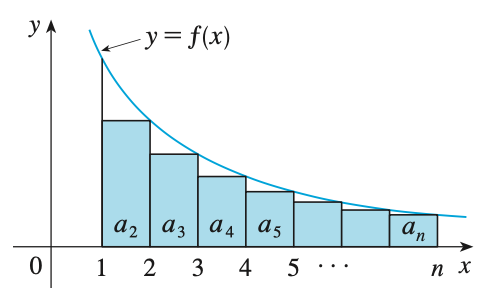
\includegraphics[width=0.4\textwidth]{integral_test1.png}
      \end{center}
      The area of the first shaded rectangle is $f(2)=a_2$. Because there is always space underneath the curve, the sum of the area of the shaded triangles from 1 to $n$ is always less than the area under the curve (since $f$ is decreasing).
      $$ a_2 + a_3 + \cdots + a_n \leq \int_{1}^{n} f(x)\ dx$$
      If $\int_{1}^{\infty} f(x)\ dx$ is convergent, then
      $$ \sum_{i=2}^{n} a_i \leq \int_{1}^{n} f(x)\ dx \leq \int_{1}^{\infty} f(x)\ dx $$
      since $f(x) \geq 0$. Therefore,
      $$ s_n = a_1 + \sum_{i=2}^{n} a_i \leq a_1 + \int_{1}^{\infty} f(x)\ dx = M \quad \text{(random variable)}$$
      Since $s_n \leq M$ for all $n$, the sequence $\{s_n\}$ is bounded above. Also
      $$ s_{n+1} = s_n + a_{n+1} \geq s_n $$
      since $a_{n+1} = f(n+1) \geq 0$. Thus, $\{s_n\}$ is an increasing bounded sequence so it it convergent by the Monotonic Sequence Theorem. This means that $\sum a_n$ is convergent.
      \item[(ii)] \textbf{Divergence}
      \begin{center}
        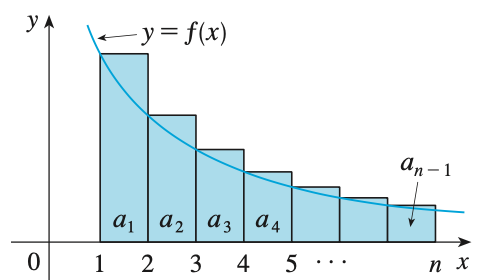
\includegraphics[width=0.4\textwidth]{integral_test2.png}
      \end{center}
      Because there is always space above the curve, the sum of the area of the shaded triangles from 1 to $n$ is always greater than the area under the curve.
      $$ \int_{1}^{n} f(x)\ dx \leq a_1 + a_2 + \cdots + a_{n-1}$$
      If $\int_{1}^{\infty} f(x)\ dx$ is divergent, then $\int_{1}^{n} f(x)\ dx \to \infty$ as $n\to\infty$ because $f(x)\geq0$. But
      $$ \int_{1}^{n} f(x)\ dx \leq \sum_{i=1}^{n-1} a_i = s_{n-1} $$
      so $s_{n-1} \to \infty$. This implies that $s_n \to \infty$ so $\sum a_n$ is diverges.
    \end{enumerate}
  \end{proof}
  \begin{example}
  Test the series $\displaystyle\sum_{n=1}^{\infty} \frac{1}{n^2 +1}$ for convergence or divergence.
  \end{example}
  \begin{solution}
    The function $f(x) = 1/(x^2 + 1)$ is continuous, positive, and decreasing on $[1,\infty)$ so we use the Integral Test:
    \begin{align*}
      \int_{1}^{\infty} \frac{1}{x^2 + 1}\ dx &= \lim_{t\to\infty} \int_{1}^{t} \frac{1}{x^2 + 1}\ dx = \lim_{t\to\infty} \tan^{-1} x \Big]_{1}^{t} \\
      &= \lim_{t\to\infty} \left(\tan^{-1} t - \frac{\pi}{4}\right) = \frac{\pi}{2}-\frac{\pi}{4} = \frac{\pi}{4}
    \end{align*}
    Thus, $\int_{1}^{\infty} \frac{1}{x^2 + 1}\ dx$ is a convergent integral. The series $\sum 1/(n^2 +1)$ is convergent by the Integral Test.
  \end{solution}
  \begin{definition}
    The \textbf{\textit{p}-series} $\displaystyle\sum_{n=1}^{\infty} \frac{1}{n^p}$ is convergent if $p>1$ and divergent if $p\leq 1$.
  \end{definition}
  For $p=1$, the series is a harmonic series.
  \begin{proof}\let\qed\relax
    If $p<0$, then $\displaystyle\lim_{n\to\infty} \frac{1}{n^p} = 0$. If $p=0$, then $\displaystyle\lim_{n\to\infty} \frac{1}{n^p} = 1$. In either case, $\displaystyle\lim_{n\to\infty} \frac{1}{n^p} \neq 0$, so the $p$-series diverges by the Test for Divergence.\par
    If $p>0$, then the function $f(x) = \dfrac{1}{x^p}$ is clearly continuous, positive, and decreasing on $[1,\infty)$. We know that $$\int_{1}^{\infty} \frac{1}{x^p} \text{ converges if } p>1 \text{ and diverges if } p\leq 1$$
    Using the Integral Test, the series $\sum 1/n^p$ converges if $p>1$ and diverges if $0<p\leq1$.
  \end{proof}
  \begin{example}
    \hphantom{ \\}
    \begin{enumerate}
      \item[(a)] The series $$\sum_{n=1}^{\infty} \frac{1}{n^3} = \frac{1}{1^3}+\frac{1}{2^3}+\frac{1}{3^3}+\frac{1}{4^3}+\cdots$$ is convergent because it is a $p$-series with $p=3>1$.
      \item[(b)] The series $$\sum_{n=1}^{\infty} \frac{1}{n^{1/3}} = \sum_{n=1}^{\infty} \frac{1}{\sqrt[3]{n}} = 1 + \frac{1}{\sqrt[3]{2}}+\frac{1}{\sqrt[3]{3}}+\frac{1}{\sqrt[3]{4}}+\cdots$$ is divergent because it is a $p$-series with $p=\frac{1}{3}<1$.
    \end{enumerate}
    \textsc{Note} We should \textit{not} infer that the sum of the series is equal to the value of the integral from the Integral Test. In fact, $$\sum_{n=1}^{\infty} \frac{1}{n^2} = \frac{\pi^2}{6} \quad\text{whereas}\quad \int_{n}^{\infty} \frac{1}{n^2}=1$$
    Therefore, in general, $$\sum_{n=1}^{\infty} a_n \neq \int_{n}^{\infty} f(x)\ dx$$
  \end{example}
  \begin{example}
    Determine whether the series $\displaystyle\sum-{n=1}^{\infty} \frac{\ln n}{n}$ converges or diverges.
  \end{example}
  \begin{solution}
    The function $\frac{\ln x}{x}$ is positive and continous for $x>1$ because the logarithm function is continuous, but it is not obvious whether or not $f$ is decreasing, so we take its derivative:
    $$ f'(x) = \frac{(1/x)x - \ln x}{x^2} = \frac{1-\ln x}{x^2}$$
    Thus, $f'(x) < 0$ when $\ln x > 1$, which is when $x > e$. We conclude that $f$ is decreasing when $x > e$ so we can apply the Integral Test:
    \begin{align*}
      \int_{1}^{\infty} \frac{\ln x}{x}\ dx &= \lim_{t\to\infty} \int_{1}^{t}\frac{\ln x}{x}\ dx = \lim_{t\to\infty} \frac{(\ln x)^2}{2}\Bigg]_{1}^{t} \\
      &= \lim_{t\to\infty} \frac{(\ln t)^2}{2} = \infty
    \end{align*}
    Since this improper integral is divergent, the series $\sum (\ln n)/n$ is also divergent by the Integral Test.
  \end{solution}
  \subsection*{Estimating the Sum of a Series}
    We can show if a series $\sum a_n$ is converging. Now we want to find an approximation to the sum $s$ of the series. ANy partial sum $s_n$ is an approximation to $s$ because $\lim_{n\to\infty} s_n = s$, but \textit{how good is that approximation}? To find out, we need to estimate the size of the \textbf{remainder}
    $$R_n = s - s_n = a_{n+1} + a_{n+2} + a_{n+3} + \cdots $$
    The remainder $R_n$ is the \textit{error} made when $s_n$, the sum of the first $n$ terms, is used as an approximation of the total sum.
    \begin{definition}[\textbf{Remainder Estimate for the Integral Test}]
      Suppose that $f(k) = a_k$, where $f$ is a continuous, positive, decreasing function for $x\geq n$ and $\sum a_n$ is convergent. If $R_n = s - s_n$, then
      $$ \int_{n+1}^{\infty} f(x)\ dx \leq R_n \leq \int_{n}^{\infty} f(x)\ dx$$
    \end{definition}
    \begin{proof}\let\qed\relax
      We use the same concept as the Integral test, assuming that $f$ is decreasing on $[n,\infty)$.
      \begin{center}
        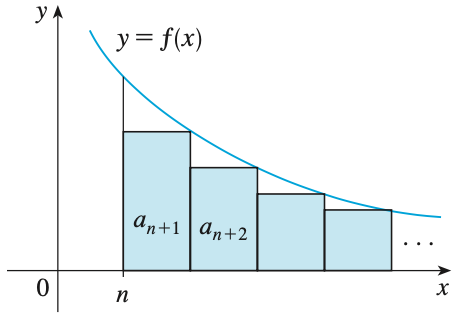
\includegraphics[width=0.4\textwidth]{estimate_sum1.png}
      \end{center}
      We compare the sum of the area of the rectangles with the area under $y=f(x)$ for $x>n$ to see that
      $$ R_n = a_{n+1} + a_{n+2} + \cdots \leq \int_{n}^{\infty} f(x)\ dx$$
      \begin{center}
        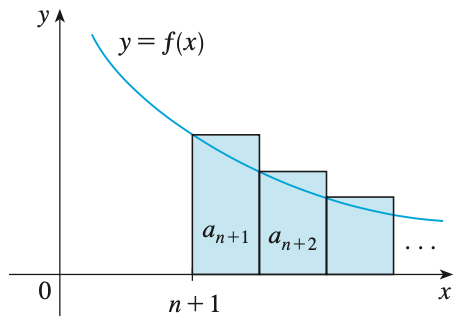
\includegraphics[width=0.4\textwidth]{estimate_sum2.png}
      \end{center}
      Similarly, we see that
      $$ R_n = a_{n+1} + a_{n+2} + \cdots \geq \int_{n}^{\infty} f(x)\ dx$$
    \end{proof}
    \begin{example}
      \begin{enumerate}
        \item[(a)] Approximate the sum of the series $\sum 1/n^3$ by using the sum of the first 10 terms. Approximate the error involved in the approximation.
        \item[(b)] How many terms are required to ensure that the sum is accurate to within 0.0005?
      \end{enumerate}
    \end{example}
    \begin{example}
      \begin{enumerate}
        $$ \int_{n}^{\infty} \frac{1}{x^3}\ dx = \lim_{t\to\infty} \left[-\frac{1}{2x^2}\right]_{n}^{t} = \lim_{t\to\infty} \left(-\frac{1}{2t^2} + \frac{1}{2n^2}\right) = \frac{1}{2n^2}$$
        \item[(a)] $$\sum_{n=1}^{\infty} \frac{1}{n^3} \approx \frac{1}{1^3} + \frac{1}{2^3} + \frac{1}{3^3} + \cdots + \frac{1}{10^3} \approx 1.1975$$
        According to the remainder estimate, we have
        $$ R_{10} \leq \int_{10}^{\infty} \frac{1}{x^3}\ dx = \frac{1}{2(10)^2} = \frac{1}{200} $$
        So the size of the error is at most 0.005.
        \item[(b)] Accuracy to within 0.0005 means that we have to find a value of $n$ such that $R_n \leq 0.0005$. Since
        $$ R_n \leq \int_{10}^{\infty} \frac{1}{x^3}\ dx = \frac{1}{2n^2}$$
        $$ \frac{1}{2n^2} \leq 0.0005 \leqno \hbox{We want}$$
        Solving this inequality, we get
        $$ n^2 > \frac{1}{0.001} = 1000 \quad\text{or}\quad n>\sqrt{1000} \approx 31.6 $$
        We need 32 terms to ensure accuracy to within 0.0005.
      \end{enumerate}
    \end{example}
    If we add $s_n$ to each side of the inequality of the Remainder Estimate for the Integral Test, we get
    \begin{definition}
      $$s_n + \int_{n+1}^{\infty} f(x)\ dx \leq s \leq s_n + \int_{n}^{\infty} f(x)\ dx$$
    \end{definition}
    because $s_n+R_n=s$. These inequalities give a lower bound and an upper bound for $s$. They provide a more accurate approximation than the partial sum $s_n$ does.
    \begin{example}
      Use the improved remainder estimate with $n=10$ to estimate the sum of the series $\displaystyle\sum_{n=1}^{\infty} \frac{1}{n^3}$.
    \end{example}
    \begin{solution}
      $$ s_{11} + \int_{11}^{\infty} \frac{1}{x^3}\ dx \leq s \leq s_{10} + \int_{10}^{\infty} \frac{1}{x^3}\ dx $$
      We know from the previous example that $$ \int_{n}^{\infty} \frac{1}{x^3}\ dx = \frac{1}{2n^2} $$
      $$ s_{11} + \frac{1}{2(11)^2} \leq s \leq s_{10} + \frac{1}{2(10)^2}  \leqno \hbox{so}$$
      Using $s_{10} \approx 1.197532$, we get $$1.201664 \leq s \leq 1.202532$$
      If we approximate $s$ by the midpoint of this interval, then the error is at most half the length of the interval, so
      $$ \sum_{n=1}^{\infty} \frac{1}{n^3} \approx 1.2021 \quad\text{with error}< 0.0005$$
      We get a much better estimate with this method than the estimate $s \approx s_n$ in the previous example. Also, we only had to use 10 terms to get the error smaller than 0.0005 instead of 32 terms.
    \end{solution}